\chapter{Entwicklung von Erweiterungen} \label{extending}

Das Java Medical Imaging Toolkit bietet sowohl dem Enwickler, als auch dem Anwender den Spielraum, die Anwendung zu erweitern. Dieses Kapitel beschreibt die Entwicklung verschiedener Plug-ins in zwei- und dreidimensionalem Raum. Zusätzlich zeigt eine Implementierung eines Werkzeugs und der Entwurf eines neuen Moduls wie die Basisfunktionen von jMediKit erweitert werden.

\section{Entwicklung von Plug-ins}

\subsection{Konventionen}

\section{Erweiterung der Anwendungsstruktur mit dem Eclipse Application Model}
Als Beispiel für eine Erweiterung soll im \textit{PartStack} des \textit{DicomBrowsers} ein neuer \textit{Part} hinzugefügt werden der theoretisch alle verfügbaren PACS im Netzwerk anzeigt. Implementiert wird nur eine minimale Oberfläche.\\
Bevor die Struktur erweitert werden kann, muss entsprechend der Anleitung in Anhang \ref{install_eclipse} die Eclipse-Installation vorbereitet sein. Sind die drei Projekte im \textit{Project Explorer} vorhanden, kann mit der Erweiterung begonnen werden.\\
Im Projekt \textit{org.jmedikit.plugin} befindet sich die Datei \textit{Application.e4xmi}\footnote{Die XML-Datei Application.e4xmi kann auch direkt im Quelltext bearbeitet werden. Die Darstellung in Eclipse erhöht die Benutzerfreundlichkeit zur Anpassung der Werte}. Darin sind alle strukturellen Informationen zu der Anwendungsoberfläche, Menüs, Handler, Commands und die Referenzen auf die implementierenden Klassen hinterlegt. Mit einem Doppelklick kann diese geöffnet werden und es zeigt sich ein Fenster wie in Abbildung \ref{e4xmi}. Die linke Spalte zeigt die Applikationsstruktur und rechts sind die entsprechenden Eigenschaften des gewählten Elements zu sehen. Ab dem Element \textit{Windows} im Strukturbaum werden die Anwendungsteile angezeigt. Dieser Teilbaum entspricht der Abbildung \ref{hierarchy} aus Kapitel \ref{architecture}. Da der \textit{PartStack} in dem der \textit{DicomBroweser} liegt erweitert werden soll, muss bis zu diesem Knoten navigiert werden. Der richtige \textit{PartStack} hat die Id \textit{org.jmedikit.plugin.dicombrowserStack}.
\begin{figure}[H]
  \vspace{0.5cm}
  \centering
  \fbox{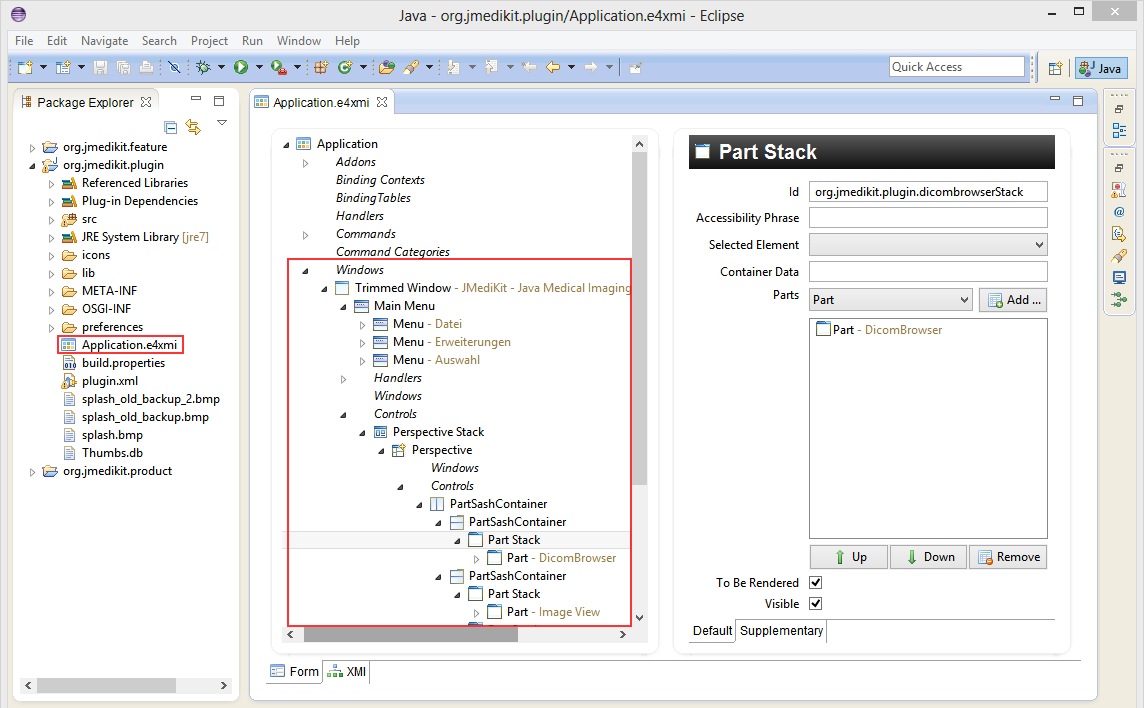
\includegraphics[angle=0,width=8cm]{./img/part_exmi.png}}
   \caption{Die Datei Application.e4xmi}
  \label{e4xmi}
  \vspace{0.5cm}
\end{figure}

Nach der Auswahl des \textit{PartStack}-Elements sind rechts dessen Eigenschaften inklusive einer Liste aller enthaltenen \textit{Parts} zu sehen(Abbildung \ref{partadd}). Über das Formularfeld \textit{Parts} kann mit einem Klick auf \textit{Add} ein neuer Kindknoten eingefügt werden. Im diesem Beispiel wird dem Stack ein neuer \textit{Part} untergeordnet.

\begin{figure}[H]
  \vspace{0.5cm}
  \centering
  \fbox{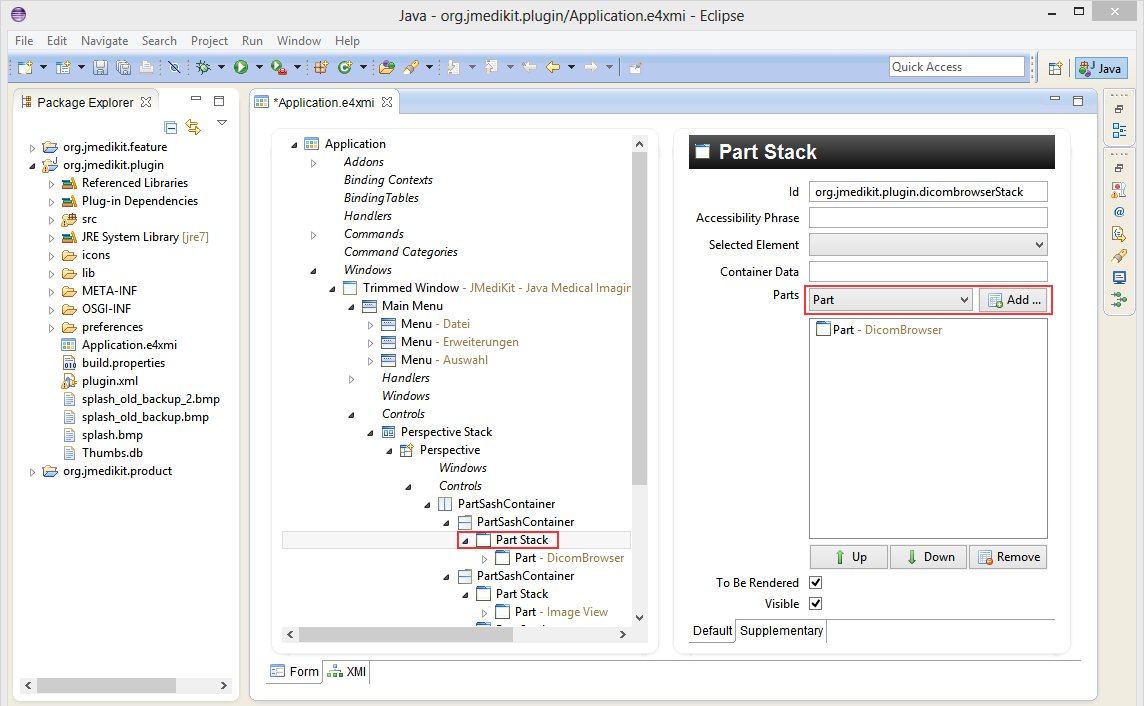
\includegraphics[angle=0,width=8cm]{./img/part_add.png}}
   \caption{Einfügen der Part-Struktur}
  \label{partadd}
  \vspace{0.5cm}
\end{figure}

Folgend öffnen sich rechts die Eigenschaften des neu angelegten Parts. Wichtige Einstellungen sind \textit{Id}, \textit{Label} und \textit{ClassURI}. Mit Hilfe der Id kann der Part im Quelltext referenziert werden und das Label ist der sichtbare Titel des \textit{Parts} in der Anwendung. Noch ist keine Klasse für das neue Strukturelement definiert worden. Dies kann mit einem Klick auf \textit{ClassURI} erledigt werden. Soll ein Icon neben dem Titel erscheinen, muss zuvor eine Bilddatei nach der Anleitung in Anhang \ref{importicon} importiert werden\footnote{Grundsätzlich ist es ausreichend die Bilddateien im \textit{icon}-Ordner zu speichern, aufgrund einer durchgehenden Konsistenz ist es allerdings besser das Bild komplett zu importieren}.

\begin{figure}[H]
  \vspace{0.5cm}
  \centering
  \fbox{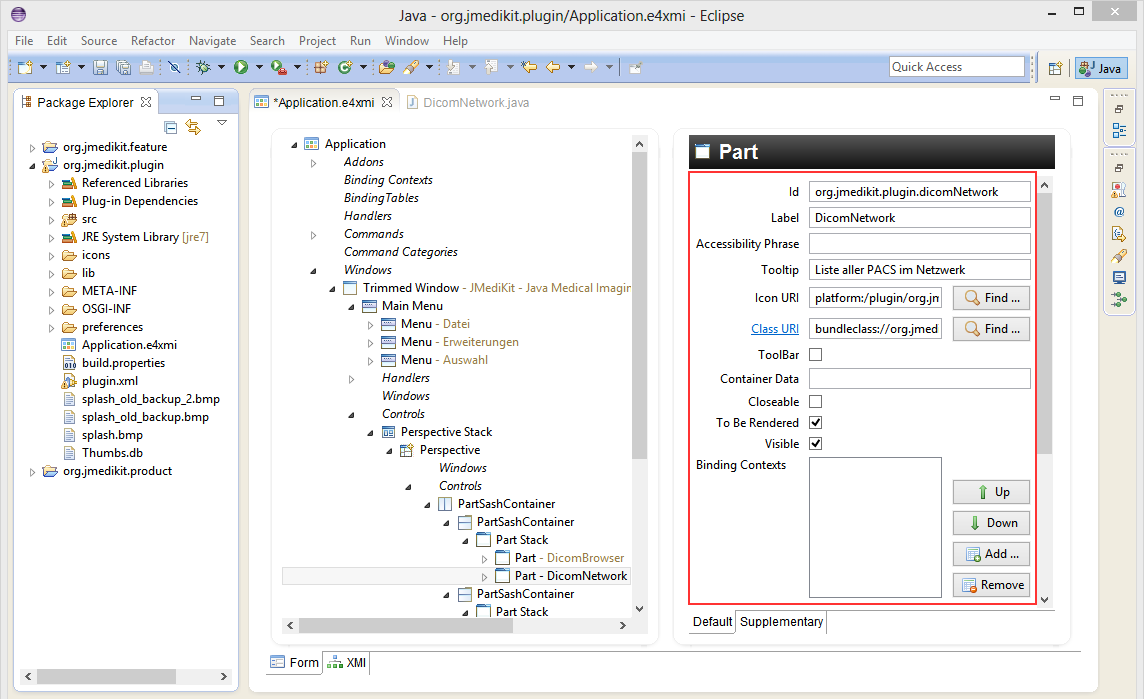
\includegraphics[angle=0,width=8cm]{./img/part_part.png}}
   \caption{Einfügen der Part-Struktur}
  \label{partpart}
  \vspace{0.5cm}
\end{figure}

Die zu erstellende Klasse repräsentiert neben der Benutzeroberfläche auch die Logik hinter dem \textit{Part}. Abbildung \ref{partclass} zeigt den Dialog zum Erstellen dieser Klasse. Alle \textit{Part}-Implementierungen befinden sich im Package \textit{org.jmedikit.plugin.gui}. Der Name ist frei wählbar. Neben Package und Klassenname kann aus vier vordefinierten Methoden gewählt werden.

\begin{figure}[H]
  \vspace{0.5cm}
  \centering
  \fbox{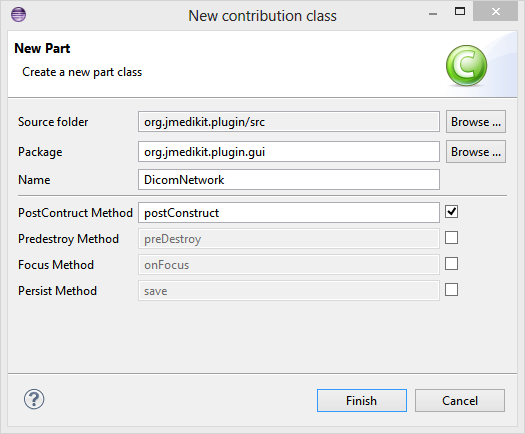
\includegraphics[angle=0,width=6cm]{./img/part_class.png}}
   \caption{Erstellen der Klasse}
  \label{partclass}
  \vspace{0.5cm}
\end{figure}

Listing \ref{partexample} zeigt eine Beispielimplementierung des \textit{Parts}. Die Annotation \textit{@PostConstruct} sorgt dafür, dass die Methode automatisch nach dem Instantiieren des Objekts ausgelöst wird. Diese enthält als Paramter ein \textit{Composite} und stellt den Einhängepunkt für die weitere Benutzeroberfläche dar.

\lstset{
language=Java,
caption={Erweiternder Eintrag einer Konstanten in der Klasse \textit{ImageProvider}},
label=partexample,
xleftmargin=1em,
xrightmargin=1em,
numbers=left,
backgroundcolor=\color{lgrey},
}  
\begin{figure}[htbp]
\begin{lstlisting}[frame=leftline]
//imports

public class DicomNetwork {

  @PostConstruct
  public void postConstruct(Composite parent) {
	
    //definiert das Layout des Elternelements
    //2 Spalten mit gleicher Breite
    GridLayout pGrid = new GridLayout(2, true);
    GridData parentData = new GridData(
        GridData.FILL_HORIZONTAL
    );
    parent.setLayout(pGrid);
    parent.setLayoutData(parentData);

    //GUI

    //Suchfeld
    Text search = new Text(parent, SWT.BORDER);
    
    //Suchbutton
    Button button = new Button(parent, SWT.NONE);
    button.setText("Suche PACS");	
  }	
}
\end{lstlisting}
\end{figure}

Abbildung \ref{partfinal} zeigt den neuen \textit{Part} in der linken Spalte der Anwendung. Damit wurde dem \textit{PartStack} in dem der \textit{DicomBrowser} enthalten ist das neue \textit{DicomNetwork} eingefügt.

\begin{figure}[H]
  \vspace{0.5cm}
  \centering
  \fbox{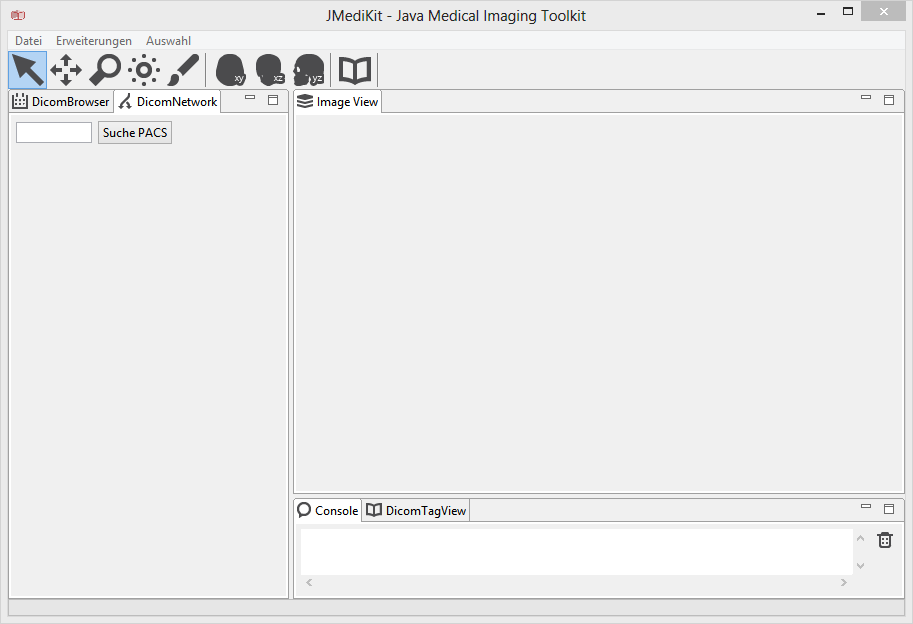
\includegraphics[angle=0,width=8cm]{./img/part_final.png}}
   \caption{Anzeige des Parts im PartStack}
  \label{partfinal}
  \vspace{0.5cm}
\end{figure}

\section{Erweiterung der Werkzeuge}
Im folgenden Abschnitt wird der Werkzeugleiste ein weiteres Tool hinzugefügt. Ähnlich dem \textit{PointTool} sollen Bildbereiche ausgewählt werden. Der Unterschied besteht darin, dass keine Punkte bestimmt werden, sondert ein rechteckiger Bildbereich als \textit{Region Of Interest}(ROI) markiert werden kann. Damit werden die Selektionswerkzeuge um das \textit{ROITool erweitert}.\\

\subsection{Hinzufügen eines Menüpunktes}

Das Menü selbst befindet sich im Applikationsbaum \textit{Window} unter dem Element \textit{TrimBars} $\rightarrow$ \textit{WindowTrim - Top} $\rightarrow$ \textit{ToolBar} und enthält \textit{HandledToolItems}-Strukturen des Application Models als Menüpunkte (Abbildung \ref{toolmenu}). Das bedeutet, dass zu jedem Eintrag ein \textit{Command} mit dem zugehörigen \textit{Handler} erstellt werden muss.

\begin{figure}[H]
  \vspace{0.5cm}
  \centering
  \fbox{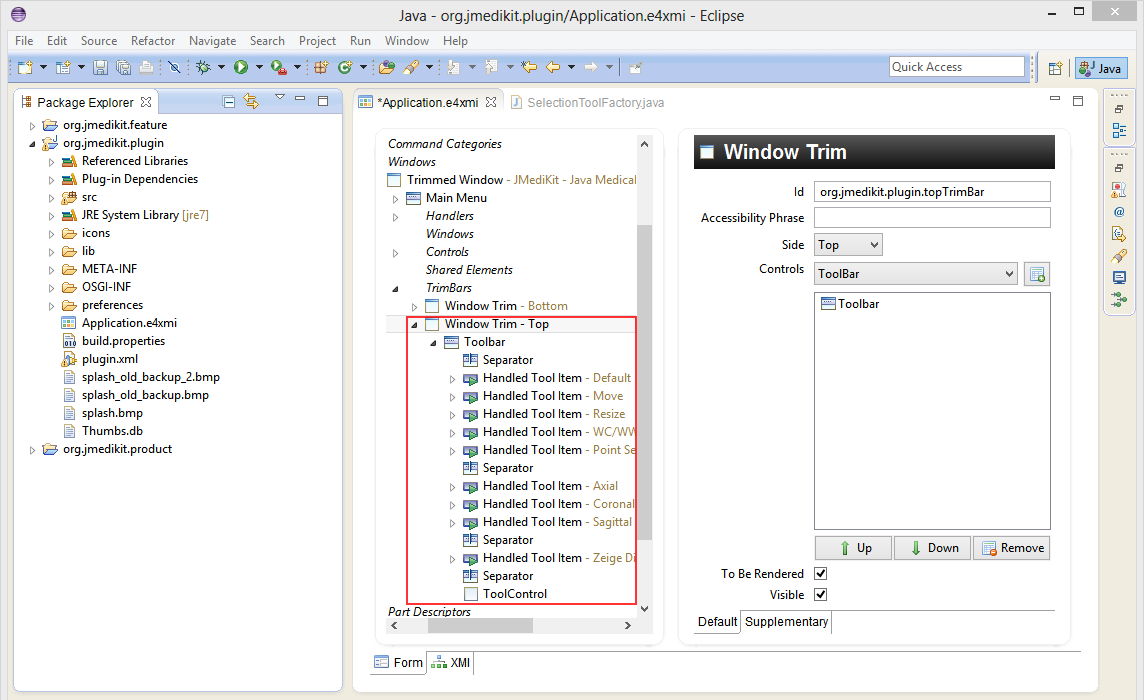
\includegraphics[angle=0,width=8cm]{./img/tool_menu.png}}
   \caption{Die Werkzeugleiste im Application Model}
  \label{toolmenu}
  \vspace{0.5cm}
\end{figure}

Die \textit{Commands} sind im Strukturbaum direkt unter \textit{Application} zu finden. Wird das Element ausgewählt, erscheint auf der rechten Seite eine Liste bisher verfügbarer \textit{Commands}. Meinem Klick auf \textit{Add} kann ein neues hinzugefügt werden. In den nun angezeigten Einstellungen bekommt die \textit{Id} den Wert \textit{org.jmedikit.plugin.command.toolRoi} und als \textit{Name} wird \textit{toolRoi} eingetragen.\\
Die Implementierung der Befehle finden in den \textit{Handlern} statt. Diese sind im Baum unter \textit{Window} angesiedelt. Nach der Auswahl erscheint die Liste der erstellten \textit{Handler}. Wie schon bei den \textit{Commands} wird ein neuer \textit{Handler} hinzugefügt und \textit{Id} sowie \textit{Name} vergeben. Unter dem Punkt \textit{Command} wird der zuvor erstellte Befehl angegeben. Mit einem Klick auf \textit{ClassURI} kann, wie in Abbildung \ref{tool_handlerclass} dargestellt, die entsprechende Klasse erstellt werden. Üblicherweise liegen Handlerklassen im Package \textit{org.jmedikit.plugin.gui.handler} und haben den Namen \textit{ToolNameHandler}.

\begin{figure}[H]
  \vspace{0.5cm}
  \centering
  \fbox{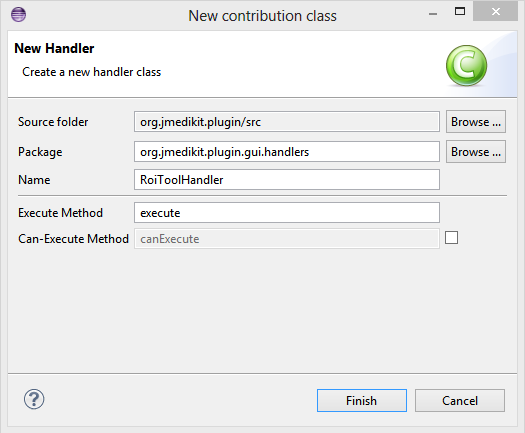
\includegraphics[angle=0,width=6cm]{./img/tool_handlerclass.png}}
   \caption{Erstellung einer Klasse für die Handlerimplementierung}
  \label{tool_handlerclass}
  \vspace{0.5cm}
\end{figure}

Im nächsten Schritt erfolgt das Hinzufügen eines \textit{HandledToolItem} zu dem Element unter \textit{Window} $\rightarrow$ \textit{TrimBars} $\rightarrow$ \textit{WindowTrim - Top} $\rightarrow$ \textit{ToolBar}. Die Reihenfolge der Liste entspricht der Darstellung in der Anwendung. Unter den Einstellungen muss \textit{Id}, \textit{Label} und \textit{Command} mit Werten belegt werden. Als \textit{Type} muss die Option \textit{Radio} gewählt werden, da genau ein Werkzeug aktiv ausgewählt sein darf. Unter dem Punkt \textit{IconURI} wird bei Bedarf ein Bild angegeben. Abbildung \ref{tool_handleditem} zeigt die gesetzten Einstellungen.

\begin{figure}[H]
  \vspace{0.5cm}
  \centering
  \fbox{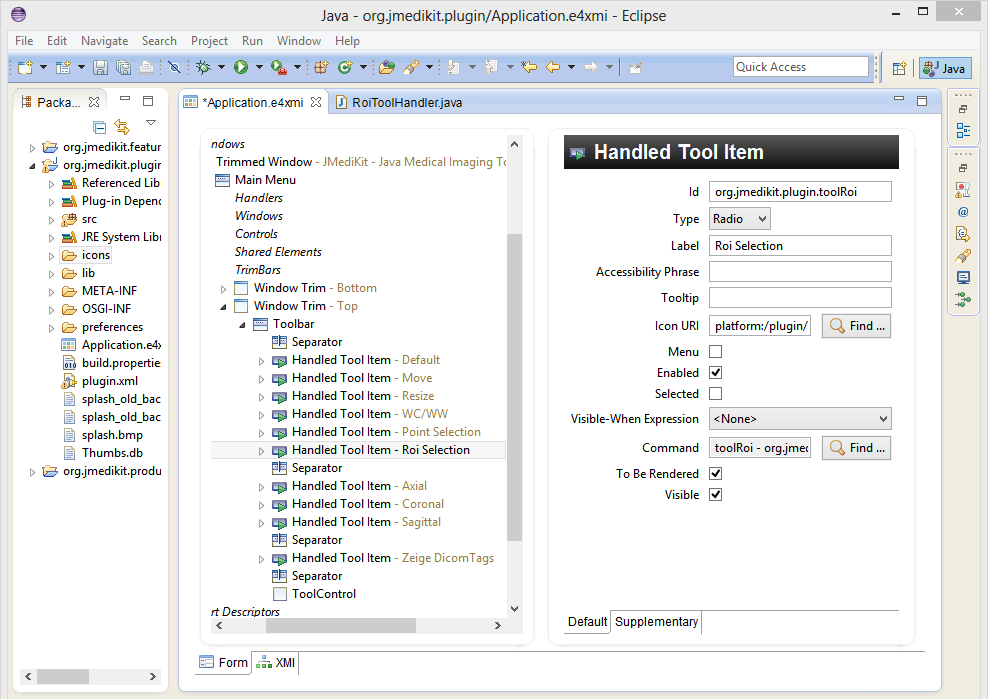
\includegraphics[angle=0,width=8cm]{./img/tool_handleditem.png}}
   \caption{Einstellungen des neuen Menüpunktes}
  \label{tool_handleditem}
  \vspace{0.5cm}
\end{figure}

Abbildung \ref{tool_menunew} zeigt die neue Werkzeugleiste mit dem \textit{ROITool} als erweiterten Eintrag.

\begin{figure}[H]
  \vspace{0.5cm}
  \centering
  \fbox{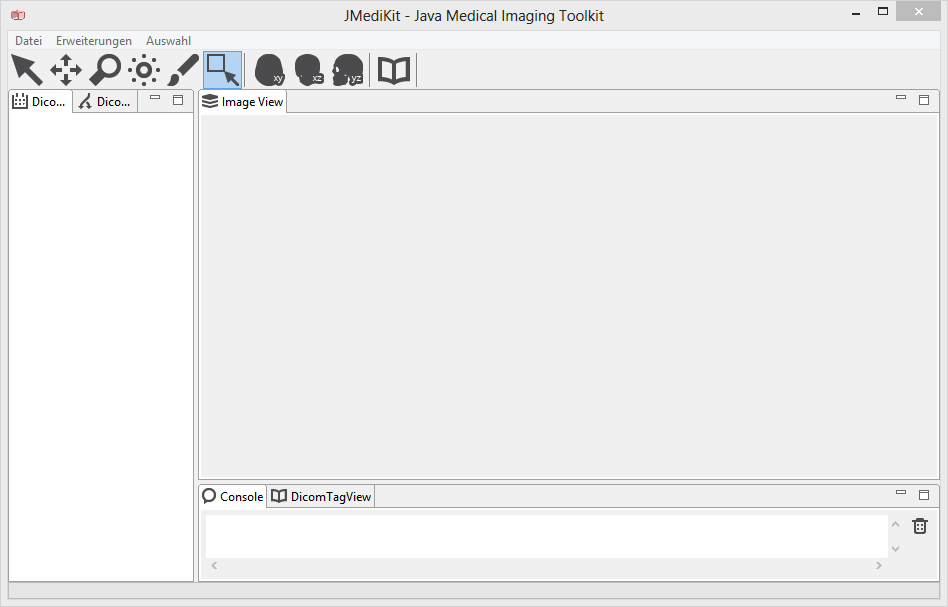
\includegraphics[angle=0,width=8cm]{./img/tool_menunew.png}}
   \caption{Anzeige der erweiterten Werkzeugleiste}
  \label{tool_menunew}
  \vspace{0.5cm}
\end{figure}

\subsection{Hinzufügen der Funktionalität}

Nach der Erweiterung der Werkzeugleiste kann die grundlegende Klasse des Werkzeugs erstellt werden. Wichtig ist die Generalisierung von \textit{ATool} wie in Listing \ref{toolclass} zu sehen ist.

\lstset{
language=Java,
caption={Erweiterung des Basiswerkzeugs},
label=toolclass,
xleftmargin=1em,
xrightmargin=1em,
numbers=left,
backgroundcolor=\color{lgrey},
}  
\begin{figure}[htbp]
\begin{lstlisting}[frame=leftline]
public class RoiTool extends ATool{

  public RoiTool(DicomCanvas c) {
    super(c);
    System.out.println("Hello ROITool");
  }
  
  //weitere Implementierungen abstrakter Methoden
  //der Klasse ATool
}
\end{lstlisting}
\end{figure}

Wird der Menüpunkt in der Werkzeugleiste betätigt, werden Events ausgelöst. In der Klasse \textit{EventConstants} sind diese jeweils in Gruppen definiert. Die Wurzel einer Gruppe hat die in Listing \ref{groups} dargestellte Struktur. \textit{TOOL\_CHANGED} ist der Gruppenname der Events, die Werkzeuge betreffen. Der Zusatz \textit{/*} symbolisiert die Wurzel. Ein spezifisches Werkzeug hat die Form \textit{TOOL\_CHANGED/TOOLNAME}. Durch die Gruppenmechanik ist es möglich, dass eine spezielle Funktion auf alle Werkzeug-Events lauscht und abhängig vom Event die Aufgaben delegiert.

\lstset{
language=Java,
caption={Eventkonstanten der Klasse EventConstants},
label=groups,
xleftmargin=1em,
xrightmargin=1em,
numbers=left,
backgroundcolor=\color{lgrey},
}  
\begin{figure}[htbp]
\begin{lstlisting}[frame=leftline]
public final static String TOOL_CHANGED_ALL = 
  "TOOL_CHANGED/*";
public final static String TOOL_CHANGED_ALL = 
  "TOOL_CHANGED/POINT";
public final static String TOOL_CHANGED_ALL = 
  "TOOL_CHANGED/ROI";
\end{lstlisting}
\end{figure}

Nachdem die Tool-Klasse und das Event kreiert wurden, kann das neue Werkzeug der Fabrik, die für die Erzeugung der Objekte zuständig ist, bekannt gemacht werden. Da das \textit{ROITool} zum Bereich der Selektion gehört, wird die Klasse \textit{SelectionToolFactory} angepasst. In Listing \ref{factory} werden die Modifikationen dargestellt. Innerhalb der Fabrik werden die zugehörigen Events in einer Konstante gespeichert. Die Methode \textit{produce} regelt die Objekterzeugung. Klickt der Anwender auf den Menüpunkt \textit{ROITool} wird das Event ausgelöst und der Werkzeugname an die Fabrik übergeben. Aufgrund des \textit{toolname} wird das richtige Werkzeug erstellt.

\lstset{
language=Java,
caption={Modifikation der SelectionToolFactory},
label=groups,
xleftmargin=1em,
xrightmargin=1em,
numbers=left,
backgroundcolor=\color{lgrey},
}  
\begin{figure}[htbp]
\begin{lstlisting}[frame=leftline]

public final static String ROI_TOOL = 
  EventConstants.TOOL_CHANGED_ROI;
//weitere Konstanten

@Override
protected ATool produce(String toolname, DicomCanvas c) {
  //Pruefung vorheriger Werkzeuge
  else if(toolname.equals(ROI_TOOL)){
    return new RoiTool(c);
  }
  //Pruefung folgender Werkzeuge
  //Werkzeug wurde nicht gefunden
  else throw new IllegalArgumentException("ERROR");
}
\end{lstlisting}
\end{figure}

Im aktuellen Zustand reagiert das Werkzeug und der neue Menüpunkt noch nicht auf die Eingaben des Benutzers. Es fehlt die Implementierung des \textit{Handlers} und die Kommunikation mit dem \textit{ImageView}. Listing \ref{roihandler} zeigt die Umsetzung der Klasse \textit{ToolRoiHandler}. Das Interface \textit{IEventBroker} regelt die Kommunikation unter den \textit{Parts}. Die Annotation \textit{@Execute} bedeutet, dass die Methode automatisch aufgerufen wird, sobald der Menüpunkt betätigt wird. Sowohl \textit{@Inject} als auch \textit{@Execute} sind Teile des \textit{Dependency Injection Frameworks} von Eclipse. Ein umfassender Artikel ist unter \cite{vogel:di} zu finden.\\
In der Methode \textit{execute} wird dem Werkzeug entsprechen die Fabrik instantiiert. Die Variable \textit{tool} enthält das auszulösende Event. Mit Hilfe des \textit{eventBroker} wird die Benutzereingabe an die lauschenden Methoden der Applikation geleitet. Die Methode \textit{post} erwartet die Event-Konstante und ein ToolEvent, welches die erzeugte Fabrik und den Werkzeugtyp als Parameter erhält.

\lstset{
language=Java,
caption={Implementierung des ToolRoiHandler},
label=roihandler,
xleftmargin=1em,
xrightmargin=1em,
numbers=left,
backgroundcolor=\color{lgrey},
}  
\begin{figure}[htbp]
\begin{lstlisting}[frame=leftline]
@Inject
IEventBroker eventBroker;

@Execute
public void execute() {

  AToolFactory factory = new SelectionToolFactory();
  String tool = EventConstants.TOOL_CHANGED_ROI;

  eventBroker.post(EventConstants.TOOL_CHANGED_ROI,
    new SelectionToolEvent(factory, tool));
}
\end{lstlisting}
\end{figure}

Klickt der Benutzer auf den Menüpunkt nachdem der \textit{Handler} implementiert wurde, erfolgt die Ausgabe \glqq Hello ROITool\grqq\ auf der Standardausgabe. Das bedeutet, das Werkzeug wurde korrekt erzeugt und kann verwendet werden. Der nächste Schritt ist die Implementierung der Logik.

\subsection{Hinzufügen der Werkzeuglogik}

Ziel des \textit{ROITools} ist es, beliebige rechteckige Flächen innerhalb des Bildes zu markieren, um diese später in Plug-ins benutzen zu können. So können Algorithmen auf ausgewählten Bildbereichen angewendet werden. Folgende Events werden von dem neuen Werkzeug behandelt:

\begin{itemize}
\item \textbf{MouseMove} \\
Bei jeder Mausbewegung wird geprüft, ob eine Maustaste gedrück wird. Ist dies der Fall, wird die Start- und die aktuelle Position solange in Datenelementen der Klasse gespeichert, bis die Taste gelöst wird.
\item \textbf{MouseDown} \\
Wird die Maustaste betätigt, werden die Koordinaten auf $0$ zurückgesetzt, damit eine neue Berechnung beginnen kann. Ohne Zurücksetzung wird die zuletzt markierte ROI nochmal auf die Zeichenfläche gemalt und bleibt bis zur ersten Mausbewegung sichtbar.
\item \textbf{MouseUp} \\
 Befindet sich nach dem Loslassen der Maustaste der Start- und Endpunkt des Cursors innerhalb des Bildes, wird eine \textit{Region Of Interest} berechnet. Dazu werden zuerst die Bildkoordinaten der beiden Punkte ermittelt. Darauf folgt eine Normalisierung der Koordinaten und ein Eintrag der im Anschluss erzeugten ROI im Bild.
\item \textbf{PostCalculation} \\
Nach der Werteberechnung wird das Rechteck der potentiellen ROI auf der Zeichenfläche dargestellt.
\end{itemize}


Ist die Logik implementiert, kann das Werkzeug in vollem Umfang eingesetzt werden. Das Erstellen von Transformationstypen erfolgt analog zu den Selektionswerkzeugen. Eine erweiterte Implementierung des \textit{ROITools} könnte zum Beispiel eine dynamische Größenanpassung der Fläche mit dem Mausrad realisieren.
%Nachdem dem Erstellen des Menüeintrags kann die Fabrik, die für die Erzeugung der Werkzeuge verantwortlich %ist, erweitert werden.